\input{preamble}
\usepackage{tikz}
\usetikzlibrary{shapes,arrows}
%\usetikzlibrary{decorations.pathreplacing}

\title{Interpretation of GLMs}

\date[]{April 21, 2015}

\begin{document}

\frame{\titlepage}

\frame{\tableofcontents}

\section{Essay 2}


\frame{
    \frametitle{Feedback on Essay 2}
    \begin{itemize}\itemsep1em
    \item Overall, these were ``OK'' but not great
    \item Issues mainly related to interpretation
    \item Other issues outlined in the email I sent
    \item Review a few of these quickly
    \end{itemize}
}

\frame{
    \frametitle{Direct Interpretation of Coefficients}
    \begin{itemize}\itemsep1em
    \item With an interaction, we cannot directly interpret the coefficients as \textit{unconditional marginal effects}
    \item Take for example:\\
        $y = 10 + 3x + 2z + 0.5 x*z$
    \item There is no ``direct'' of effect of $x$ or ``direct'' effect of $z$
    \item Don't use this language (direct/indirect) effects at all!
    \item Instead, think about effect \textit{heterogeneity}
    \end{itemize}
}

\frame{
    \frametitle{Direct Interpretation of Coefficients}
    \begin{itemize}\itemsep1em
    \item It can be problematic to interpret coefficients on an interaction term
    \item A lot of assignments talked about an interaction meaning that an effect was ``larger'' or ``smaller''
    \item This is tough because a positive coefficient estimate can mean:
        \begin{itemize}
        \item A larger positive effect of $x$ if $\beta_x$ is positive
        \item A smaller positive effect of $x$ if $\beta_x$ is negative
        \item A larger negative effect of $x$ if $\beta_x$ is negative
        \item Some combination of the above
        \end{itemize}
    \end{itemize}
}
    
    
\frame{
    \frametitle{Hypotheses}
    \begin{itemize}\itemsep1em
    \item Don't hypothesize the size of the coefficient estimate on the interaction term
    \item Instead: hypothesize the pattern of effect heterogeneity and the levels of the outcome across different values of the causally important variables
    \item Don't interpret the estimates on variables that you are not theoretically interested in
        \begin{itemize}
        \item Ex. Interested in the effect of education on trust
        \item You condition on gender as a possible confounder
        \item You do not hypothesize the ``effect'' of gender
        \item Do not say anything about its coefficient estimate
        \end{itemize}
    \end{itemize}
}



\begin{frame}[fragile]
    \frametitle{A ``Heuristic'' Graph}
	\begin{center}
	\begin{tikzpicture}[>=latex',circ/.style={draw, shape=circle, node distance=5cm, line width=1.5pt}]
        \draw[->] (0,0) node[left] (X) {X} -- (5,0) node[right] (Y) {Y};
        \draw[-] (X) -- (2.5,0) node[right] (D) {};
        \draw[->] (3.1,0) -- (5,0) (Y);
        \draw[->] (-2,2) node[left] (Z) {Z} -- (Y);
        \draw[->] (Z) -- (X);
        \draw[->] (2.5,-1) node[below] (M) {M} -- (D);
    \end{tikzpicture}
    \end{center}
\end{frame}
% causal graphs vs. linear path models vs. ``heuristic'' theoretical drawings

\begin{frame}<0>[fragile]
    \frametitle{Better: Two Causal Graphs}
	\begin{center}
	\begin{tikzpicture}[>=latex',circ/.style={draw, shape=circle, node distance=5cm, line width=1.5pt}]
        \draw[->] (0,0) node[left] (X1) {X} -- (2,0) node[right] (Y1) {Y};
        \draw[->] (-1,2) node[left] (Z1) {Z} -- (Y1);
        \draw[->] (Z1) -- (X1);
        \draw[->] (0,-2) node[left] (M1) {M} -- (Y1);

        \draw[->] (5,0) node[left] (X2) {X} -- (7,0) node[right] (Y2) {Y};
        \draw[->] (4,2) node[left] (Z2) {Z} -- (Y2);
        \draw[->] (Z2) -- (X2);
        \draw<1>[->] (5,-2) node[left] (M2) {M} -- (Y2);
    \end{tikzpicture}
    \end{center}
\end{frame}



\begin{frame}[fragile]
    \frametitle{Representing Theory as Graph}
	\begin{center}
	\begin{tikzpicture}[>=latex',circ/.style={draw, shape=circle, node distance=5cm, line width=1.5pt}]
        \draw[->] (0,0) node[left] (X) {X} -- (4,0) node[right] (Y) {Y};
        \draw[-] (X) -- (2.5,0) node[right] (D) {};
        \draw[->] (3.1,0) -- (Y);
        \draw[->] (-1,2) node[left] (Z) {Z} -- (Y);
        \draw[->] (Z) -- (X);
        \draw<2->[->] (0,-2) node[left] (M) {M} -- (Y);
        \draw<2>[->] (Z) -- (M);
        \draw<3->[->] (3,-3) node[below] (W) {W} -- (Y);
        \draw<3->[->] (W) -- (M);
    \end{tikzpicture}
    \end{center}
\end{frame}


\frame{
    \frametitle{Interpretation}
    \begin{itemize}\itemsep1em
    \item<1-> How do we interpret a coefficient estimate in a regression model with no interaction terms?
    \item<2-> How do we interpret a coefficient estimate in a regression model with one or more interaction terms?
    \item<3-> How do we calculate predicted or fitted values from our estimates?
    \item<4-> How can we visually display the results of a regression estimation?
    \end{itemize}
}

\frame{
    \frametitle{Graphing Activity}
    \begin{itemize}\itemsep1em
    \item It can be difficult to see regression without results without graphing them
    \item But, using Stata it can be unclear how the estimated regression equation conforms to particular graphical output
    \item So, you will practice graphing \textit{by hand}
    \item Do activities \# 1--3
    \end{itemize}
}









\section{Review GLMs and MLE}
\frame{\tableofcontents[currentsection]}


\frame{
    \frametitle{Non-continuous Outcomes}
    \begin{enumerate}\itemsep1em
    \item Why shouldn't we use OLS for a non-continuous outcome variable?
    \item<2-> What do we do instead?
        \begin{itemize}
        \item<3-> Use a generalized linear model (GLM)
        \end{itemize}
    \end{enumerate}
}


\frame{
    \frametitle{Regression on a Latent Variable}
    \begin{itemize}\itemsep1em
    \item Consider a binary outcome $y$ (e.g., voting)
    \item OLS provides a nonsensical fit to the outcome
    \item Think about the problem as a ``latent'' outcome ($y\ast$) that manifests in two observed categories
        \begin{itemize}
        \item As $y\ast$ increases, $Pr(Y=1) \rightarrow 1$
        \item As $y\ast$ decreases, $Pr(Y=1) \rightarrow 0$
        \end{itemize}
    \item We do not observe $y\ast$, only $y$
    \end{itemize}
}

\frame{
    \frametitle{Estimation in GLM}
    \begin{itemize}\itemsep1em
    \item In OLS, we estimate: $\hat{y} = \beta_0 + \beta_1 x + e$
    \item This represents the conditional mean of $y$
    \item In a GLM, we estimate: $\hat{y}\ast = \beta_0 + \beta_1 x + e$\\
    where $y\ast$ is a transformation of $y$
    \item This is also a prediction of the conditional mean of $y$
    \item<2-> How do we transform $y$ to $y\ast$?
    \end{itemize}
}

\frame{
    \frametitle{Model Specification}
    \begin{enumerate}\itemsep1em
    \item<1-> Complete set of conditioning variables
    \item<2-> Correctly specified model
    \item<3-> Choice of error distribution
    \item<4-> Link function
    \end{enumerate}
}

\frame{
	\frametitle{Error Distribution}
	\begin{itemize}\itemsep1em
	\item To estimate a linear model using OLS, no distributional assumption is needed
	\item We can use Maximum Likelihood Estimation to obtain identical coefficient estimates as OLS by assuming errors are Normally distributed
    	\begin{itemize}
    	\item $\dfrac{1}{\sigma\sqrt{2\pi}} e^{-\dfrac{(x-\mu)^2}{2\sigma^2}}$
    	\end{itemize}
	\item For any GLM, we must assume the population distribution of the errors
    	\begin{itemize}
    	\item In almost all cases, an \textit{exponential family} distribution
    	\item i.e., a bell-shaped distribution that is not Normal
    	\end{itemize}
	\end{itemize}
}


\frame{
    \frametitle{Link Function}
    \begin{itemize}\itemsep2em
    \item $y\ast = X\beta = \beta_0 + \beta_1 x_1 + \beta_2 x_2 + \dots$
    \item \textbf{Link function}: $g(\mu) = X\beta$
        \begin{itemize}
        \item Transforms $y$ to $y\ast$
        \end{itemize}
    \item \textbf{Inverse link function}: $\mu = g^{-1}(X\beta)$
        \begin{itemize}
        \item Transforms $y\ast$ back to $y$
        \end{itemize}
    \end{itemize}
}


\begin{frame}[fragile]
    \frametitle{Inverse Link Function}
    
    \begin{itemize}
    \item This plot displays $g^{-1}(0.75x)$, where $g^{-1}$ is the inverse logit link.
    \end{itemize}
    
    \begin{center}
    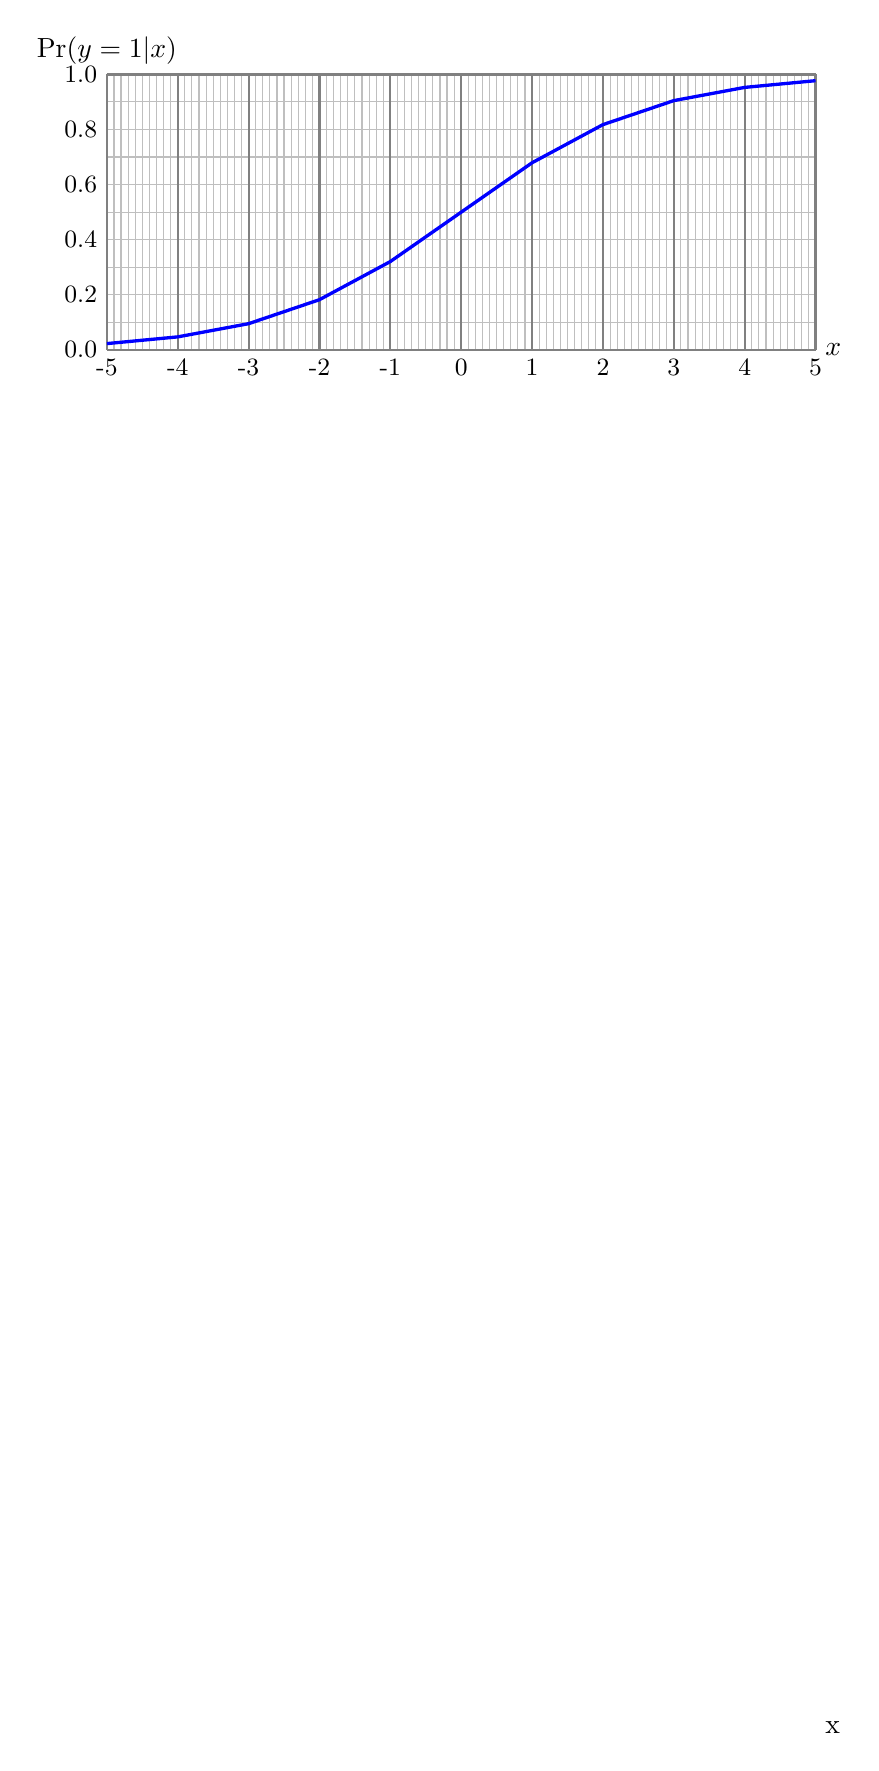
\begin{tikzpicture}[yscale=3.5, xscale=0.9]
    \draw [thin, step=0.1, lightgray] (-5,0) grid (5,1);
    \draw [thick, gray] (-5,0) grid (5,1);
    \node[right] () at (5,-5) {x};
    \node[right] () at (5,0) {$x$};
    \node[above] () at (-5,1) {$\Pr(y=1|x)$};
    \foreach \x in {-5,...,5} {
        \node[below] () at (\x,0) {\small \x};
    }
    \foreach \y in {0.0,0.2,0.4,0.6,0.8,1.0} {
    \node[left] () at (-5,\y) {\small \y};
    }
    % paste0("(", -5:5, ",", round(plogis(0.75*(-5:5)),4), ")", collapse = " -- ")
    \draw [very thick, blue] (-5,0.023) -- (-4,0.0474) -- (-3,0.0953) -- (-2,0.1824) -- (-1,0.3208) -- (0,0.5) -- (1,0.6792) -- (2,0.8176) -- (3,0.9047) -- (4,0.9526) -- (5,0.977);
    \end{tikzpicture}
    \end{center}
\end{frame}

\begin{frame}[fragile]
    \frametitle{From $x$ to Linear Prediction ($y\ast$)}
    \begin{center}
    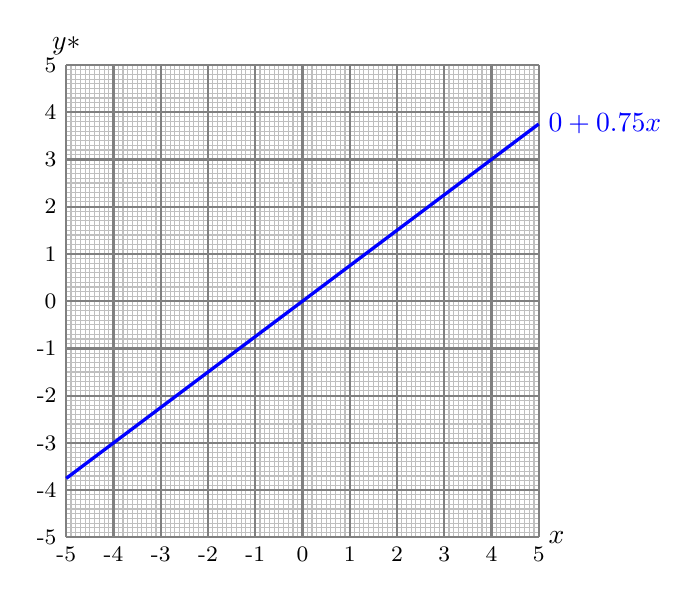
\begin{tikzpicture}[scale=0.6]
    \draw [thin, step=0.1, lightgray] (-5,-5) grid (5,5);
    \draw [thick, gray] (-5,-5) grid (5,5);
    \node[right] () at (5,-5) {$x$};
    \node[above] () at (-5,5) {$y\ast$};
    \foreach \x in {-5,...,5} {
        \node[below] () at (\x,-5) {\footnotesize \x};
    }
    \foreach \y in {-5,...,5} {
    \node[left] () at (-5,\y) {\footnotesize \y};
    }
    % paste0("(", -5:5, ",", round(0.75*(-5:5),4), ")", collapse = " -- ")
    \draw [very thick, blue] (-5,-3.75) -- (-4,-3) -- (-3,-2.25) -- (-2,-1.5) -- (-1,-0.75) -- (0,0) -- (1,0.75) -- (2,1.5) -- (3,2.25) -- (4,3) -- (5,3.75);
    \node[right,blue] () at (5,3.75) {$0 + 0.75x$};
    \end{tikzpicture}
    \end{center}
\end{frame}


\begin{frame}[fragile]
    \frametitle{From $y\ast$ to $Pr(y=1)$}
    \begin{center}
    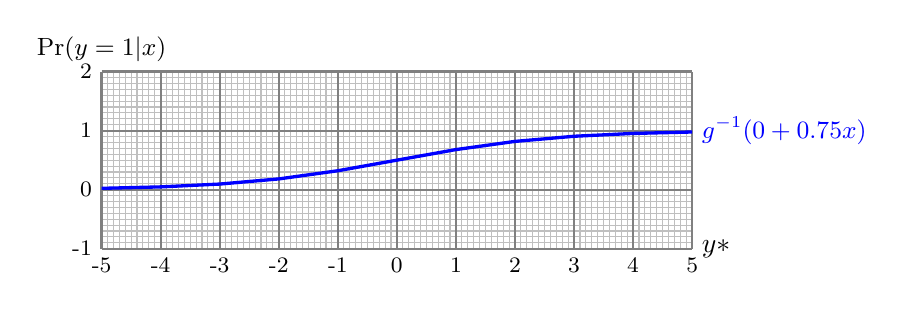
\begin{tikzpicture}[scale=0.75]
    \draw [thin, step=0.1, lightgray] (-5,-1) grid (5,2);
    \draw [thick, gray] (-5,-1) grid (5,2);
    \node[right] () at (5,-1) {$y\ast$};
    \node[above] () at (-5,2) {\small $\Pr(y=1|x)$};
    \foreach \x in {-5,...,5} {
        \node[below] () at (\x,-1) {\footnotesize \x};
    }
    \foreach \y in {-1,...,2} {
    \node[left] () at (-5,\y) {\footnotesize \y};
    }
    % paste0("(", -5:5, ",", round(plogis(0.75*(-5:5)),4), ")", collapse = " -- ")
    \draw [very thick, blue] (-5,0.023) -- (-4,0.0474) -- (-3,0.0953) -- (-2,0.1824) -- (-1,0.3208) -- (0,0.5) -- (1,0.6792) -- (2,0.8176) -- (3,0.9047) -- (4,0.9526) -- (5,0.977);
    \node[right,blue] () at (5,1) {\small $g^{-1}(0 + 0.75x)$};
    \end{tikzpicture}
    \end{center}
    
    \begin{itemize}
    \item Function is monotonic
    \item There is a \textit{cutpoint} in $y\ast$ where $\Pr(y) = 0.5$
    \item It is symmetric above and below the cutpoint
    \end{itemize}
\end{frame}


\begin{frame}[fragile]
    \frametitle{Putting it Together}
    \vspace{-1.5em}
    \begin{center}
    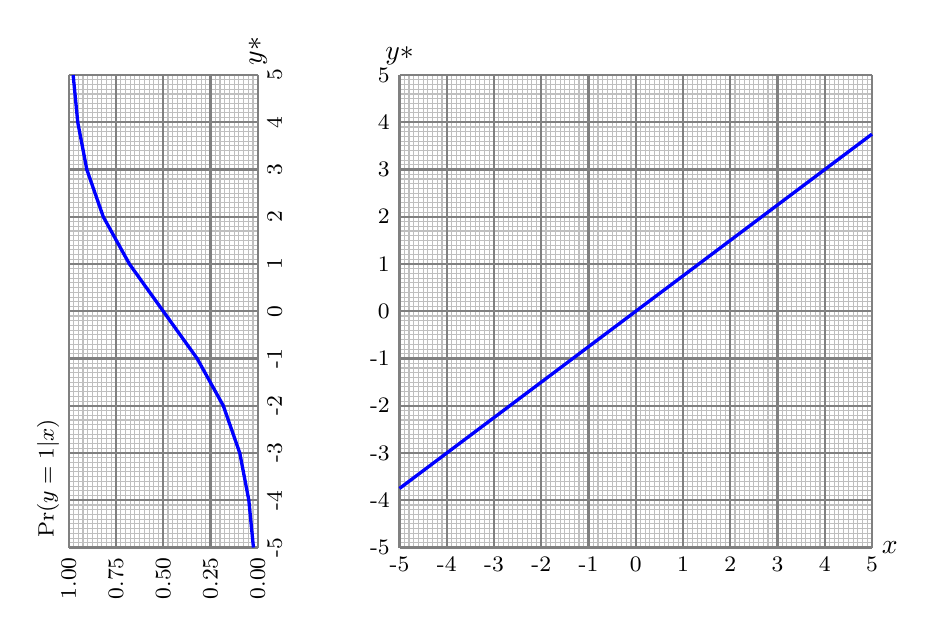
\begin{tikzpicture}[scale=0.6]
    
    % Pr(y)
    \draw [thin, step=0.1, lightgray] (-12,-5) grid (-8,5);
    \draw [thick, gray] (-12,-5) grid (-8,5);
    \node[left,rotate=90] () at (-8,-5) {\footnotesize 0.00};
    \node[left,rotate=90] () at (-9,-5) {\footnotesize 0.25};
    \node[left,rotate=90] () at (-10,-5) {\footnotesize 0.50};
    \node[left,rotate=90] () at (-11,-5) {\footnotesize 0.75};
    \node[left,rotate=90] () at (-12,-5) {\footnotesize 1.00};
    \foreach \y in {-5,...,5} {
        \node[below,rotate=90] () at (-8,\y) {\footnotesize \y};
    }
    \node[right,rotate=90] () at (-8,5) {$y\ast$};
    \node[above right,rotate=90] () at (-12,-5) {\footnotesize $\Pr(y=1|x)$};
    % paste0("(", -(8 + 4*round(plogis(0.75*(-5:5)),4)), ",", -5:5, ")", collapse = " -- ")
    \draw [very thick, blue] (-8.092,-5) -- (-8.1896,-4) -- (-8.3812,-3) -- (-8.7296,-2) -- (-9.2832,-1) -- (-10,0) -- (-10.7168,1) -- (-11.2704,2) -- (-11.6188,3) -- (-11.8104,4) -- (-11.908,5);
        
    % y*
    \draw [thin, step=0.1, lightgray] (-5,-5) grid (5,5);
    \draw [thick, gray] (-5,-5) grid (5,5);
    \node[right] () at (5,-5) {$x$};
    \node[above] () at (-5,5) {$y\ast$};
    \foreach \x in {-5,...,5} {
        \node[below] () at (\x,-5) {\footnotesize \x};
    }
    \foreach \y in {-5,...,5} {
        \node[left] () at (-5,\y) {\footnotesize \y};
    }
    % paste0("(", -5:5, ",", round(0.75*(-5:5),4), ")", collapse = " -- ")
    \draw [very thick, blue] (-5,-3.75) -- (-4,-3) -- (-3,-2.25) -- (-2,-1.5) -- (-1,-0.75) -- (0,0) -- (1,0.75) -- (2,1.5) -- (3,2.25) -- (4,3) -- (5,3.75);
    %\node[right,blue] () at (5,3.75) {$0 + 0.75x$};
    \end{tikzpicture}
    \end{center}
\end{frame}


\frame{
	\frametitle{Choosing a Link Function}
	\begin{itemize}\itemsep1em
	\item Based on expected distribution of the error term of $y\ast$
	\item Choice heavily influenced by convention rather than empirics
	\item Choice of link adds \textit{model dependence}!
		\begin{itemize}
		\item Expected influence of $x$ on $y$ now depends on choice of link
		\item Different link functions can yield different substantive and statistical results
		\item Generally, results are similar
		\end{itemize}
	\end{itemize}
}


\frame{
    \frametitle{Common Link Functions}
    \begin{center}
    {\renewcommand{\arraystretch}{1.75}
    \begin{tabular}{p{1in} p{1in} p{1in}}
    \textit{Name} & \textit{Link} & \textit{Inverse} \\ \hline
    Identity & $\mu$ & $y\ast$ \\
    Logit & $\ln\dfrac{\mu}{1-\mu}$ & $\dfrac{1}{1+e^{-y\ast}}$ \\
    Probit & $\Phi^{-1}(\mu)$ & $\Phi(y\ast)$ \\
    \hline
    \end{tabular}
    }
    \end{center}
    
    \begin{itemize}
    \item These are common for categorical outcomes
    \item Other types of outcomes will use different link functions
    \end{itemize}
}

\frame{
    \frametitle{Modelling: Price and Zaller}
    \begin{itemize}\itemsep1em
    \item Recall the Price and Zaller article from last week
    \item What is their theory?
    \item How do they test that theory?
    \item How much do their results depend on modeling decisions?
    \end{itemize}
}

\frame{
    \frametitle{Beyond Binary Outcomes}
    \begin{itemize}\itemsep1em
    \item The generalized linear model works for all kinds of outcomes, not just continuous or binary
    \item Consider, for example, a multi-category, ordered outcome variable
    \item In an \textit{ordered logit} model, we imagine a latent variable $y\ast$ and multiple cutpoints between categories of $y$
    \end{itemize}
}


\frame{\frametitle{Questions about GLMs?}}


\frame{
    \frametitle{Maximum Likelihood Estimation}
    \begin{itemize}\itemsep1em
    \item The \textit{generalized linear model} is a way of describing complex regression models
    \item Unlike OLS, there is no closed-form mathematical solution to GLM
        \begin{itemize}
        \item Recall a linear model can be expressed as a GLM
        \end{itemize}
    \item GLMs involve the big additional assumption of a distribution for the error term
    \item Maximum likelihood estimation is a way of estimating the GLM that makes use of that error distribution
    \end{itemize}    
}

\frame{
    \frametitle{Maximum Likelihood Estimation}
    \begin{itemize}\itemsep1em
    \item Choose an error distribution (which is described by various parameters)
    \item Select parameters as starting values
    \item Give a \textit{probability} of seeing each observation in our sample data given that distribution
    \item Combine those probabilities (i.e., likelihoods)
        \begin{itemize}
        \item Multiply the likelihoods
        \item Add the log-likelihoods
        \end{itemize}
    \item Repeat and pick the best guess from all of those that we test
    \end{itemize}
}


% assumptions



\frame{\frametitle{Questions about MLE?}}


\section{Interpreting GLMs}
\frame{\tableofcontents[currentsection]}

\frame{
    \frametitle{Coefficients}
    \begin{itemize}\itemsep1em
    \item Coefficients express effect of $x$ on $y\ast$
    \item In logistic regression, this is a statement about the odds-ratio:
        $\hat{\beta} = \dfrac{\frac{p_1}{1-p_1}}{\frac{p_0}{1-p_0}}$
    \item Coefficients are hard to interpret \textit{substantively}
    \item Statistical significance is similar to OLS
    \end{itemize}
}

\frame{
    \frametitle{Predicted Outcomes}
	\begin{itemize}\itemsep1em
	\item In OLS, fitted values from the estimated regression equation are values of $y$
	\item In GLMs, fitted values are expressed for $y\ast$
	\item To interpret logit or probit, we transform to predicted probabilities
	\end{itemize}
}

\frame{
    \frametitle{Predicted Outcomes}
	\begin{itemize}\itemsep1em
	\item Definition: According to our coefficient estimates, what is $\Pr(\hat{y} = 1|X)$?
	\item To calculate this, we:
    	\begin{enumerate}
    	\item Calculate a fitted value on the latent/linear scale
    	\item Plug that fitted value into the inverse link function
    	\end{enumerate}
    \item In Stata, use \texttt{margins} and \texttt{predict}
        \begin{itemize}
        \item Probabilities are the default
        \item Use the \texttt{, xb} option for linear predictions
        \end{itemize}
    \end{itemize}
}


\frame{
    \frametitle{Marginal Effects}
    \begin{itemize}\itemsep1em
    \item A marginal effect refers to one of two quantities:
        \begin{itemize}
        \item For continuous variables: the partial derivative of the regression equation with respect to a specific variable
        \item For categorical variables: the difference $\Pr(y=1|x=1) - \Pr(y=1|x=0)$
        \end{itemize}
    \item In an OLS (with no interactions or other complex terms), the marginal effect is the coefficient itself
    \item In GLMs, this is more complicated
    \end{itemize}
}


\frame{
    \frametitle{Review: Partial Derivatives}
    \begin{itemize}\itemsep1em
    \item The partial derivative is the \textit{instantaneous} slope (or \textit{tangent}) of a line
    \item With one $x$ variable, this is just the slope of the line
    \item With > 1 $x$ variable, this is the conditional slope of the regression surface
        \begin{itemize}
        \item We hold other variables at some value see a ``slice'' of the regression surface
        \item The marginal effect is the slope of the slice
        \end{itemize}
    \end{itemize}
}


\frame{
	\frametitle{Simple regression surface}
	\begin{center}
	\begin{tikzpicture}
	    \draw[thick,->] (0,0,0) -- (6,0,0) node[anchor=north east]{$x$};
	    \draw[thick,->] (0,0,0) -- (0,4,0) node[anchor=north west]{$y$};
	    \draw[thick,->] (0,0,0) -- (0,0,5) node[anchor=south]{$z$};
	    \filldraw[draw=red,fill=red!20,opacity=0.5]
	        (0,2,0) -- (0,0,4) -- (5,-2,4) -- (5,0,0) -- cycle;
	    \draw<1> (3,3,0) node {$\hat{y} = \hat{\beta}_0 + \hat{\beta}_1 X + \hat{\beta}_2 Z$};
        \draw<2> (3,3,0) node {$\dfrac{\partial y}{\partial Z} = \hat{\beta}_2$};
	    \draw<2>[thick, red] (0,2,0) -- (0,0,4);
	    \draw<3> (3,3,0) node {$\dfrac{\partial y}{\partial X} = \hat{\beta}_1$};
	    \draw<3>[thick, blue] (0,2,0) -- (5,0,0);
	\end{tikzpicture}
	\end{center}
}



\frame{
    \frametitle{Graphing Activity (cont.)}
    \begin{itemize}\itemsep1em
    \item Do graphing activity \# 4
    \end{itemize}
}

\frame{
    \frametitle{Discrete Changes}
    \begin{itemize}\itemsep1em
    \item Marginal effects are \textit{instantaneous changes}
    \item This makes sense for continuous variables
    \item For categorical (factor) variables, we often instead calculate a discrete change\\
        \begin{itemize}\itemsep1em
        \item $Pr(y=1|x=1) - Pr(y=1|x=0)$
        \item Marginal effect and discrete change are the same in OLS
        \end{itemize}
    \end{itemize}
}

\frame{
    \frametitle{Graphing Activity (cont.)}
    \begin{itemize}\itemsep1em
    \item Do graphing activity \# 5
    \end{itemize}
}

\frame{
    \frametitle{Interaction Terms}
    \begin{itemize}\itemsep1em
    \item Due to the link function transformation, the marginal effect of $x$ depends on the value of $x$ and all other covariates
    \item This creates \textit{implicit} interactions
    \item We still have to include \textit{explicit} interaction terms to estimate heterogeneous effects (i.e., effect moderation)
    \end{itemize}
}


\frame{
    \frametitle{Graphing Activity (cont.)}
    \begin{itemize}\itemsep1em
    \item Do graphing activities \# 6--7
    \end{itemize}
}


\frame{
	\frametitle{Logit vs. Probit}
	\begin{itemize}\itemsep1em
	\item<1-> Both constrain a continuous $y\ast$ to (0,1)
	\item<2-> Probabilities are symmetric
	\item<3-> Logit allows us to estimate odds-ratios
	\item<4-> Logit is maybe slightly more common in political science for what are probably just historical reasons
	\end{itemize}
}

\frame{
    \frametitle{Graphing Activity (cont.)}
    \begin{itemize}\itemsep1em
    \item Do graphing activity \# 8
    \end{itemize}
}

\frame{
    \frametitle{Language of Interpretation}
    \begin{itemize}\itemsep1em
    \item How do we describe a marginal effect in OLS?
    \item<2-> In a binary outcome model, we use different language\\
    \item<3-> The substantive importance of an effect may depend on the level of $\Pr(y)$ at which it occurs\\
        \begin{itemize}\itemsep1em
        \item<4-> Small effect at $\Pr(y) = 0.01$ vs. $\Pr(y) = 0.48$
        \item<5-> Large positive effect when $\Pr(y)$ is always $> 0.6$
        \end{itemize}
    \item<6-> Substantive importance depends on variability and \textit{stickiness} of $x$
    \end{itemize}
}


\frame{\frametitle{Questions?}}


\frame{
    \frametitle{Summarizing Marginal Effects}
    \begin{itemize}\itemsep1em
    \item We need to decide the values for all covariates that we will use in summarizing the marginal effect of our focal variable
    \item If our equation is: $y = g^{-1}(\beta_0 + \beta_1 x_1 + \beta_2 x_2 + \dots)$
    \item And we want to know the marginal effect of $x_1$, we need to hold $x_2$ at some specified value(s)
    \end{itemize}
}

\frame{
    \frametitle{3 Common Marginal Effect Summaries}
    \begin{enumerate}\itemsep2em
    \item Marginal Effects at the Mean (MEMs)
    \item Marginal Effects at Representative Values (MERs)
    \item Average Marginal Effects (AMEs)
    \end{enumerate}
}


\frame{
    \frametitle{MEM}
    \begin{itemize}\itemsep1em
    \item We are interested in the ME of $x_1$
    \item We hold all other covariates at their respective means
    \item For example, we interested in the ME of \textit{knowledge}, we hold \textit{education} at its mean
    \item<2-> Does this make sense for categorical values (e.g., gender)?
    \end{itemize}
}

\frame{
    \frametitle{MERs}
    \begin{itemize}\itemsep1em
    \item The means of the covariates may not be meaningful
    \item We hold those covariates at various interesting values
        \begin{itemize}
        \item ME of $x$ for a high-school educated female
        \item ME of $x$ for a university-educated male
        \item etc.
        \end{itemize}
    \item Helpful because we may also be interested in $\Pr(y=1)$ for these cases
    \end{itemize}
}

\frame{
    \frametitle{AMEs}
    \begin{itemize}\itemsep1em
    \item We may not only be interested in MEs at particular values
    \item We may want a summary measure of the effect of $x$ for our sample as a whole
    \item The \textit{average marginal effect} calculates the MER for every observation in our data, then averages those ME values
    \item This is Stata's default behavior when using:\\ \texttt{margins, dydx(*)}
    \end{itemize}
}


\frame{
    \frametitle{AMEs: An Example}
    \begin{itemize}
    \item Model effects of gender \& education on trust
    \item Calculate ME for each observation
    \item Average to obtain AME
    \end{itemize}
    
    \visible<2->{
    \begin{center}
    \begin{tabular}{lllrr}
    Obs. & Gender & Degree & $ME(Gender)$ & $ME(Degree)$ \\
    \hline 
    1 & 1 & 1 & 0.10 & 0.25 \\
    2 & 1 & 1 & 0.10 & 0.25 \\
    3 & 1 & 0 & 0.20 & 0.15 \\
    4 & 0 & 1 & 0.30 & -0.25 \\
    5 & 0 & 0 & 0.10 & -0.40 \\
    \hline 
    AME & -- & -- & \only<3->{0.16} & \only<4->{0.00} \\
    \hline 
    \end{tabular}
    \end{center}
    }
}

\frame{
    \frametitle{Statistical Uncertainty}
    \begin{itemize}\itemsep1em
    \item Always express statistical uncertainty for:
        \begin{itemize}
        \item Coefficients
        \item Predicted probabilities
        \item Marginal effects
        \end{itemize}
    \item Significance of coefficients and marginal effects may vary
    \item Marginal effects may only differ from 0 on a subset of the range of $x$
    \item Be cautious about extrapolation
    \end{itemize}
}


\frame{
    \frametitle{Aside: Discrete Effects}
    \begin{itemize}\itemsep1em
    \item Discrete effects can also be calculated for continuous variables
    \item Requires choosing a substantively meaningful change in $x$
    \item \textbf{Caution!} Not necessary equal:\\
        \begin{itemize}\itemsep1em 
        \item $\Pr(y = 1|x = 5) - \Pr(y = 1|x = 1)$
        \item ME at $x = 5$ (MER)
        \item ME at $x = 1$ (MER)
        \item ME at $x = 3$ (AME/MEM)
        \end{itemize}
    \end{itemize}
}

\begin{frame}[fragile]
    \frametitle{Discrete and Marginal Effects}
    \vspace{-1.5em}
    \begin{center}
    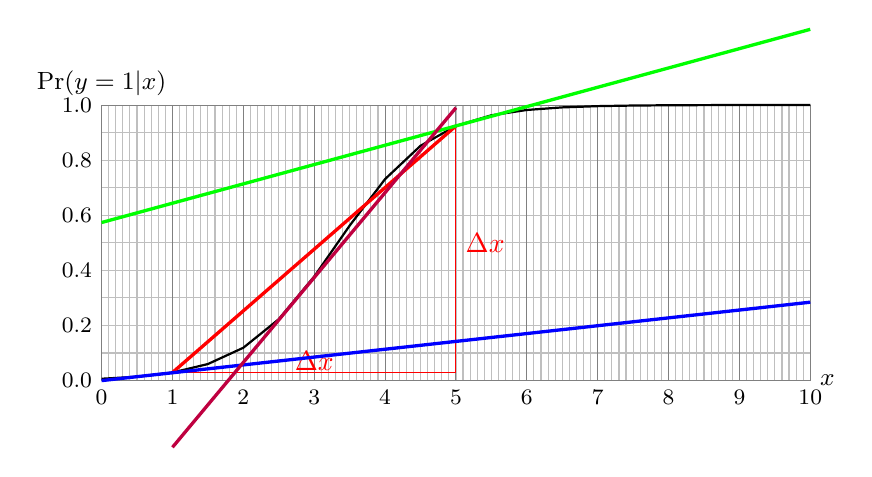
\begin{tikzpicture}[yscale=3.5, xscale=0.9]
    \draw [thin, step=0.1, lightgray] (0,0) grid (10,1);
    \draw [thin, gray] (0,0) grid (10,1);
    \node[right] () at (10,0) {\small $x$};
    \node[above] () at (0,1) {\small $\Pr(y=1|x)$};
    \foreach \x in {0,...,10} {
        \node[below] () at (\x,0) {\footnotesize \x};
    }
    \foreach \y in {0.0,0.2,0.4,0.6,0.8,1.0} {
    \node[left] () at (0,\y) {\footnotesize \y};
    }
    % paste0("(", seq(0,10,by=0.5), ",", round(plogis(-5 + 1.5*(seq(0,10,by=0.5))),4), ")", collapse = " -- ")
    \draw [thick, black] (0,0.0067) -- (0.5,0.0141) -- (1,0.0293) -- (1.5,0.0601) -- (2,0.1192) -- (2.5,0.2227) -- (3,0.3775) -- (3.5,0.5622) -- (4,0.7311) -- (4.5,0.852) -- (5,0.9241) -- (5.5,0.9627) -- (6,0.982) -- (6.5,0.9914) -- (7,0.9959) -- (7.5,0.9981) -- (8,0.9991) -- (8.5,0.9996) -- (9,0.9998) -- (9.5,0.9999) -- (10,1);
    
    % discrete change
    % plogis(-5 + (1.5 * 1))
    % plogis(-5 + (1.5 * 5))
    \draw<2> [red] (1,0.0293) -- (5,0.0293);
    \draw<2> [red] (5,0.0293) -- (5,0.9241);
    \draw<2> [very thick, red] (1,0.0293) -- (5,0.9241);
    \node<2>[right,red] () at (5, 0.5) {$\Delta x$};
    \node<2>[above,red] () at (3, 0) {$\Delta x$};
    
    % ME at x = 1
    % dlogis(-5 + (1.5 * 1))
    \draw<3> [very thick, blue] (0,0) -- (10,0.2845);
    
    % ME at x = 5
    % dlogis(-5 + (1.5 * 5))
    \draw<4> [very thick, green] (0,0.5736) -- (10,1.2746);
    
    % ME at x = 3
    % dlogis(-5 + (1.5 * 3))
    \draw<5> [very thick, purple] (1,-0.242) -- (5,0.99);
        
    
    \end{tikzpicture}
    \end{center}
    
    \vspace{-2em}
    
    {\small
    \begin{itemize}
    \item<2-6> Discrete change: 0.9241 - 0.0293 = 0.8948
    \item<3-6> ME at $x = 1$: 0.0285
    \item<4-6> ME at $x = 5$: 0.0701
    \item<5-6> ME at $x = 3$: 0.2350
    \end{itemize}
    }
    
\end{frame}

\frame{
    \frametitle{Language of Interpretation}
    \begin{itemize}\itemsep0.5em
    \item \textbf{Discrete effect}: A change in $x$ from $a$ to $b$ results in an increase in the predicted probability that $y$ equals 1 of 0.89, which is a substantively large and statistically significant effect.
    \item \textbf{Marginal effect}: The marginal effect of $x$ on the probability that $y$ = 1 when $x$ equals $a$ is 0.07, which is a large and statistically significant effect. The predicted probability of $y$ at this point is only 0.03, however, suggesting $x$ may be substantively unimportant for cases with this value of $x$.
    \end{itemize}
}


\frame{
    \frametitle{Interpretation: Hobolt}
    \begin{itemize}\itemsep1em
    \item Recall the Hobolt article from last week
    \item What is her research question? What is her theory?
    \item What is the test of that theory?
    \item How does she interpret the results?
    \end{itemize}
}



\frame{
    \frametitle{Summary}
    \begin{itemize}\itemsep1em
    \item Many ways to summarize GLMs
        \begin{itemize}
        \item Coefficients
        \item Predicted probabilities
        \item Marginal effects
        \item Discrete effects
        \end{itemize}
    \item<2-> Graphs help interpretation considerably
    \item<3-> There's no single correct way of summarizing a complex model
    \end{itemize}
}



\frame{\frametitle{Questions?}}


\frame{
    \frametitle{Preview}
    \begin{itemize}\itemsep2em
    \item Tomorrow: More logit and probit in Stata
        \begin{itemize}\itemsep1em
        \item Marginal effects
        \item Graphing
        \end{itemize}
    \item Next week: GLMs for non-binary outcomes
    \end{itemize}
}

\appendix
\frame{}

\end{document}
